\documentclass{article}

\usepackage{times}
\usepackage{uist}
%\usepackage[config, font=small, labelfont={sf,bf}, textfont=sf]{caption,subfig}
%\usepackage{setspace}
%\doublespace
\usepackage[config, font=small, labelfont={sf,bf}, textfont=sf]{caption}
\usepackage{subfig}
\usepackage{graphicx}

\begin{document}

% --- Copyright notice ---
%\conferenceinfo{UIST'11}{October 16-19, 2011, Santa Barbara, CA, USA}
%\CopyrightYear{2011}
%\crdata{978-1-4503-0716-1/11/10}

% Uncomment the following line to hide the copyright notice
\toappear{}
% ------------------------

\bibliographystyle{plain}

\title{Sketch It, Make It: Freehand Drawing for Precision Rapid Fabrication}

\author{
\parbox[t]{9cm}{\centering
	     {\em Author One}\\
	     Institution Name\\
             City, ST, USA\\
	     user@institution.net}
\parbox[t]{9cm}{\centering
	     {\em Author Two}\\
	     Institution Name\\
             City, ST, USA\\
	     user@institution.net}
}

\maketitle

% TODO: change this
\abstract Abstract goes here. 

\classification{I.3.5 [Computational Geometry and Object Modeling]: Modeling packages}

% TODO: change this
\terms{Design, Human Factors}

\keywords{sketching, rapid fabrication, design tools, constraints}

\tolerance=400 % prevent words from sticking out in the margin

%% \begin{figure}[tb]
%% \vspace{1.9in}
%% \caption{A figure caption.  It is set in 9 point Helvetica type, with a
%% 0.5 cm wider margin on both left and right sides.} 
%% \label{fig-example}
%% \end{figure}

\section{INTRODUCTION}

A growing community of self-described \textit{Makers} design and build
many kinds of physical things~\cite{gershenfeld-fab}. Some are
electronic or robotic gizmos, while others are made from traditional
material. These ``new makers''~\cite{gross-new-makers} are empowered
by rapid fabrication machines like 3D printers and laser
cutters. 

Laser cutters are among the more common and affordable fabrication
machines. They can be thought of as a very fast, strong, and precise
automated razor, cutting through flat material (paper, wood, plastic,
metal, etc.). Many things can be made entirely with a laser cutter,
sometimes fastened with screws or glue.
Figure~\ref{fig:laser-example} shows several examples of useful items
made with laser cutters.

\begin{figure}[b]
\centering 
\subfloat[] {
  \label{fig:laser-example-a} 
  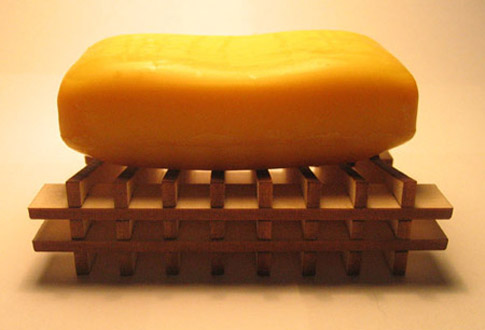
\includegraphics[width=0.4\linewidth]{img/flat-b.jpg}
}
\subfloat[] {
    \label{fig:laser-example-b}
    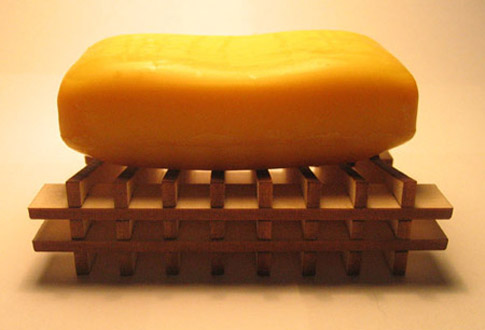
\includegraphics[width=0.4\linewidth]{img/flat-b.jpg}
}
\caption{Laser cut items.}
\label{fig:laser-example}
\end{figure}

A new sector of businesses use rapid fabrication to cater to hobbyist
designers as well as people who need highly customized goods. For
example, companies such as Ponoko fabricate physical output from
digital models that users upload over the web. 

Today, designers can choose among several modeling tools for laser
cutter projects. The most commonly used tool is Adobe Illustrator, a
general-purpose, full-featured vector graphics editor. It has an
interface new users find familiar. Despite this familiarity,
participants in our formative study had a hard time using Illustrator
quickly and effectively because they spent a great deal of effort
looking for appropriate functions among the many features that are
extraneous to laser cutters. Expert designers use specialized CAD
tools such as Rhino or SolidWorks are perhaps more appropriate for
this kind of modeling, but those tools have a substantial learning
curve. If design by end-users is to become common, appropriate
modeling tools must be made accessible to ordinary
users~\cite{lipson-homefactory}.

We present ``Sketch It, Make It'' (SIMI), a modelling tool based on
recognizing short sequences of input sketched with a stylus. Using
freehand drawn input, SIMI enables the designer to iteratively and
incrementally create laser cut models to precise specifications.

Research on sketch-based modeling tools~\cite{johnson-sketch-review}
typically see sketching as an activity done mostly in the early phases
of design. Tools based on this assumption are justifiably oriented
towards supporting inprecise input without placing undue focus on
unimportant detail. Only a few sketch-based systems support designers
in later stages when it is important to focus on precision. 

We are inspired by the potential of freehand drawing as a basis for
precision modeling for several reasons. Sketching is quick and can be
easily learned. The technology is simple and modeless: unlike
structured editing software, a designer does not need to set the
pencil's mode to line, circle, or anything else. And, a freehand
sketch can provide enough information to translate into a digital
model.

\subsection{Contributions}

This paper presents the results of a formative study on how people
design items for laser cutting. We also provide an analysis of
artifacts from Maker community web sites that reveals specific
properties common to many laser cutter projects.

The primary contribution is a system characterized by iterative,
incremental sketch-based modeling for designing precise 2D shapes
for laser cutting. Prior work on sketch-based modeling tools explored
only narrow topics in the space (like corner finding, recognition
algorithms, or mode switching). We improve on existing sketch-based
interaction techniques and bring them together in a system whose sum
is greater than its parts. The system's success depends on how well
the individual features work well together. While this might sound
trivial, it is not. We believe our system gives users a remarkably
fluid environment for designing laser cut items.

We then present results of a user study of this tool. % TODO: more...

\section{BACKGROUND}

Laser cut designs are composed of parts cut from solid, flat pieces of
material and assembled in various ways: laminated, notched, bolted
together, \textit{etc}. The primary concern of the designer is to
define the outline of parts produced with the laser
cutter. Alternately the user can design joints so the parts fit
together. Most joints have small margins of error. It is imperative
that lengths, angles, and relative position be indicated with
precision so that the parts to fit together as they should.

\section{RELATED WORK}

While ``the design process'' has important differences between
domains, two properties are common to nearly all design work,
including design for laser cutters. First, designers sketch throughout
the process, especially in the beginning. Second, a computer tool is
used to render the design more precisely. This is confirmed by
observations of graphic designers~\cite{wong-rr-prototypes},
automotive engineers~\cite{kara-styling}, and software
developers~\cite{dekel-improvised-notation}. Freehand drawing is a
powerful means for thinking and specifying design intent, but it is
disconnected from the computer aided portion of the design
process~\cite{company-sketching-in-engineering}.

\subsection{Sketch-based interaction}

% Mark says: The Related Work section should include not only projects
% about sketch-to-fab, but also representative sketch projects that
% don't address fabrication.  Although SIMI is a tool for making
% drawings for laser cutter production, it does have potential for
% broader use, and regardless, reviewers will compare it with other
% non-fab sketch systems.  Therefore the RW section may as well tackle
% SIMI in the context of sketch systems in general.

% A few of the more well-known and relevant sketching systems:

% * SILK, because it let you interact with the recognized elements of
%   the sketch

The rough appearance of freehand sketches support designers to see
past unimportant details, letting them focus on the big picture. Much
prior work argues that rectification is antagonistic to
design~\cite{gross-cocktail}, at least during the conceptual
phases. SILK is a sketch-based tool for quickly drawing user
interfaces~\cite{landay-silk-chi}. While the system recognizes user
input as UI elements like menus, scrollbars or buttons. The system
lets the designer use the recognized sketch, even as it retains its
rough appearance. Finally, SILK can translate the recognized sketch
into a working implementation.

% * Pegasus, because of interactive beautification, 2D vector drawing,
%   constraint inference. Also Murugappan's beautification thing.

% In here, I need to say something about the tradeoffs of recognizing
% too much. Systems like Pegasus and Murugappan's thing are pretty
% aggressive about inferring constraints. This leads to very nice
% looking drawings, but it also precludes the user from making things
% that can't be inferred.

Some work takes an alternate view on the appearance of sketched
input. Systems such as Pegasus~\cite{igarashi-pegasus} and recent work
by Murugappan \textit{et. al}~\cite{murugappan-beautification}
`beautify' the drawing by replacing rough input with cleaned up
graphic elements like lines or arcs. These 2D graphics systems infer
the user's intention by inferring geometric constraints. If more than
one constraint is possible, the system lets the user choose among a
small number of alternatives. These tools enable users to quickly and
easily make clean-looking vector graphics. However, the aggressive
inferencing might prevent users from making drawings that have subtle
but important features the system can not infer.

% * EverybodyLovesSketch, because it lowers the barrier for normal
%   people to create complex 3D models with a coherent set of
%   interaction techniques.

Sketch input is an appealing way to interact with computers because it
is apparently natural and easy for users to provide. Unfortunately,
sketch recognizers are not sophisticated enough to reliably interpret
drawings. Researchers have created ways to attend the gap between the
input people would like to provide and the computer's ability to make
sense of it. This is often done by asking users to draw in certain
ways (e.g. shapes must be drawn with single strokes) to conform to the
recognizer's capabilities, like in SILK. Others develop or refine
sketch-based interaction techniques that that are natural for humans
to use and easier for the computer to understand.

Teddy~\cite{igarashi-teddy} and more recently
EverybodyLovesSketch~\cite{bae-everybody} are two examples of this
second category. They both provide a small grammar of easy-to-use
gestures that people use to create and edit 3D drawings. The ease and
power of these systems is evident: children can learn and use them to
create seemingly complex models. EverybodyLovesSketch in particular
seeks to enable a broad audience to create 3D perspective conceptual
sketches by choosing a set of gestures and tools that work well
together.

\subsection{Sketch-based modeling for fabrication}

Computer support for fabrication design has been a topic of interest
for several decades, under the rubric of computer aided design
(CAD)/computer aided manufacturing (CAM). While today interaction is
mostly performed with a keyboard and mouse, this was not always the
case. For example, SketchPad~\cite{sutherland-sketchpad} users
controlled the design by setting modes and parameters with one hand
and drew directly on the screen with a light pen in the other.

More recently, novel interfaces enable users to model items for
fabrication by sketching. For example, Plushie~\cite{mori-plushie}
lets people design soft objects such as stuffed animals. Users create
3D models of bulbous objects by sketching in a manner similar to
Teddy~\cite{igarashi-teddy}. The program creates a set of 2D shapes
that users can cut from fabric, sew, and stuff.

Sketch Chair is a more recent example of a tool that makes design for
rapid fabrication more accessible~\cite{saul-sketch-chair}. Users
sketch the contours of a chair's seat and back rest, and in a
different drawing mode, add legs. The system includes a sophisticated
physical simulator to let the designer explore its physicality (for
example to determine if it will remain upright). It also allows
designers to change subtle properties of curves using on-screen
control handles.

Most work on sketch-based interfaces focuses on the early phases of
design when people are thinking about framing the problem and
solution. Sketch-based systems such as Plushie and Sketch Chair enable
people to make things they otherwise would not be able to, but the
designer relinquishes a great deal of control to the system. Further,
they support only a narrow class of artifacts.

A few sketch-based systems support
precision. ParSketch~\cite{naya-parsketch} enables designers to create
parametric 2D models by incrementally recognizing sketched geometry
and commands. It uses pressure to distinguish between linework (high
pressure) and constraint commands (lower pressure). Sketch-based
drawing tools Pegasus~\cite{igarashi-pegasus} and Lineogrammer let
users make clean, rectified vector graphics. They work on the
principle of interactive beautification, which supports iterative
sketch/rectify sequences. Many sketch-based systems invoke recognition
after the user has added a complete sketch. The interactive nature of
these precision-oriented systems means the system has less work to do
when its recognizer/rectifier is invoked. This generally leads to more
accurate recognition and higher user satisfaction.

\section{BACKGROUND STUDY}

To better understand the domain of laser cutter fabrication we
conducted two related empirical studies. We interviewed people with
experience designing these artifacts, and watched them work. From this
we form a picture of the kinds of tasks and problems designers face
when designing for laser cutters. We also analyzed laser-cut items on
community web sites to find common features.

\subsection{Formative Study on Designer Work Practices}
\label{sec:formative}

We interviewed six designers to learn about their work practices and
to understand how they use their tools. The participants had
substantially different backgrounds, but all were trained in some form
of design, including mechanical engineering, graphic design, and
architecture. The participants were part of our tool's target
demographic: people who were interested in making things with laser
cutters as a hobby.

Each session lasted approximately an hour and was split evenly between
interview and implementation. We asked participants to describe their
design process, and to show sketches or videos of their work. While
there are differences (some subtle) in their process, each followed
the same overall pattern.

They begin by thinking about a problem and sketching. Some were are
made to think about how to frame the project (what it is for), while
others help reason about how to make it (how it works, how it fits
together). Some designers explicitly noted that sketching is a
necessary part of the process; it would not be possible to move
forward without making freehand drawings. When the idea is reasonably
well-formed they will translate their hand-made sketch into a computer
model (Figure~\ref{fig:translate}).

\begin{figure}[h]
  \centering
  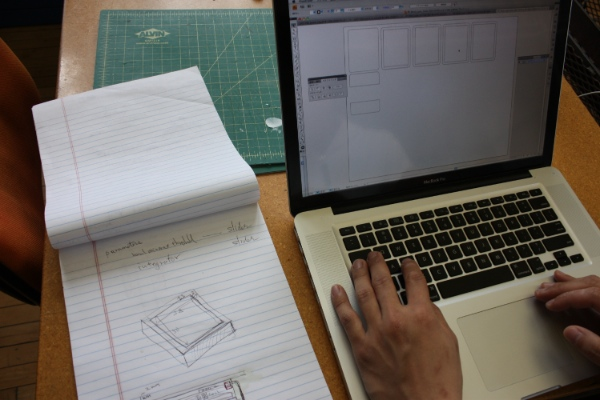
\includegraphics[width=0.9\linewidth]{img/translate-sketch-to-computer.jpg}
  \caption{A common part of designing for laser cutters: translating a
    hand-made sketch to a computer modeling tool. The sketch includes
    a perspective drawing of the desired result, and 2D diagrams of
    individual parts with key dimensions indicated.}
  \label{fig:translate}
\end{figure}

After the work practices interview, we asked participants to implement
the sketch shown in Figure~\ref{fig:interview-sketch} using a software
tool of their choice. Our purpose was to learn what problems
people encountered when executing the common task of translating a
sketch to a computer model.

\begin{figure}[h]
\centering 
\subfloat[The part users set out to replicate.] {
  \label{fig:interview-sketch-1} 
  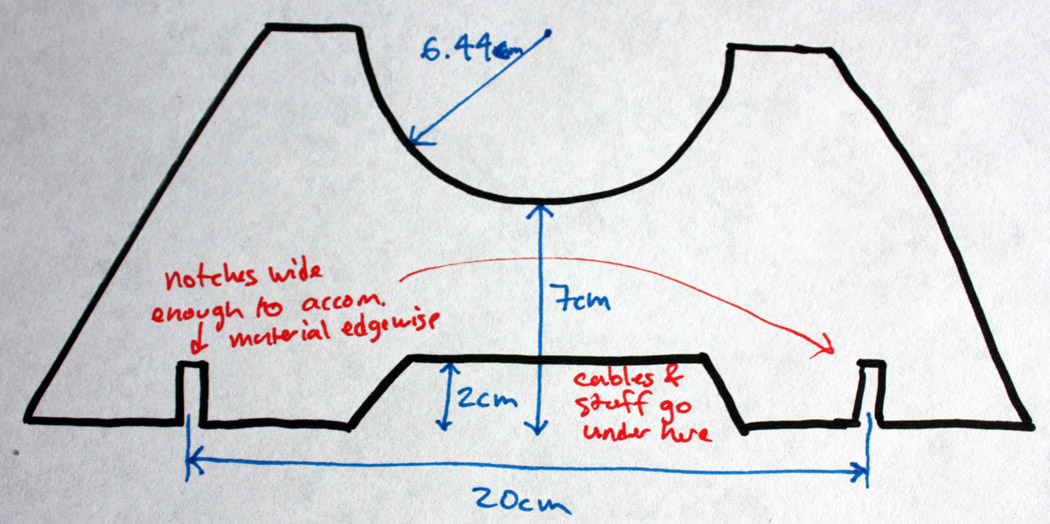
\includegraphics[width=0.9\linewidth]{img/laser-me-1.jpg}
}

\subfloat[Drawing of how the part is used in context.] {
    \label{fig:interview-sketch-2}
    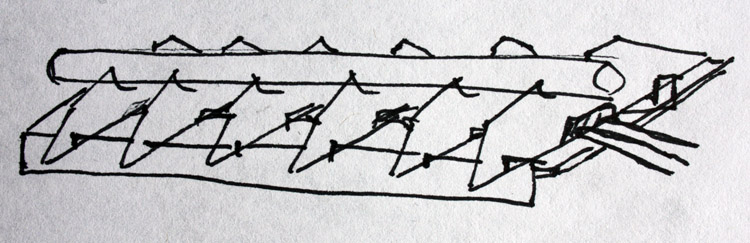
\includegraphics[width=0.9\linewidth]{img/laser-me-2.jpg}
}
\caption{Participants were asked to create the stencil at the top
  using modeling software.}
\label{fig:interview-sketch}
\end{figure}

Most participants chose to implement the sketch with Illustrator (5
users), while one chose Rhino. In all cases, the designer's strategy
involved common activities: creating or editing boundaries, aligning
or snapping items, using guide lines or reference points, measuring
distances, specifying or changing lengths and angles, and creating
finished ``cut files'' to send to the laser cutter. These
domain-specific tasks are in addition to the usual interaction
management tasks such as selecting/deselecting on-screen elements, or
view port management like zooming and panning.

Participants spent a good deal of time on operating overhead. This
includes (1) searching for the appropriate tool for the next task, (2)
recovering from errors made after selecting the wrong tool, or (3)
when the tool behavior was inconsistent with the user's
intention. Approximately 50\% of the designer's time was spent in this
way.

For example, one user was aware of Illustrator's ``Path Finder'' tool
and wanted to use it. The user searched the program's menu structure
and slowly hovered over toolbar buttons to read tool tips before
finding it. Next, the designer invoked various functions of the Path
Finder, using the keyboard shortcut to undo after each attempt, as he
searched for the correct mode within the subcommand palette. This
process lasted approximately 80 seconds before finally being able to
continue.

Occasionally participants used features in rather strange ways to
achieve a desired outcome. For example, in order to remove an unwanted
segment of a polyline, one participant (a graphic designer) created an
opaque white rectangle to obscure it, rather than erase it. (``Don't
tell anyone I did this'', he said at the time).

Similar episodes are common: a person \textit{should} know the
`correct' action, but takes an alternate approach. The alternative
might achieve the intended effect, but it might be less efficient
(more operations, longer execution time) or it might introduce
unwanted complexity (such as the invisible white rectangle).

To summarize, we found the common tasks and problems found following
our interview study:

\begin{itemize}
\item creating/editing boundaries
\item aligning/snapping items
\item using guide lines or reference points
\item measuring distances
\item specifying lengths/angles
\item creating cut files
\item selecting/deselecting
\item view port management
\item finding and entering tool modes
\item recover from error (tool or user error)
\item `correct' action is unknown or hard to do
\end{itemize}

\subsection{Artifact Analysis}

Ponoko and Thingiverse are two currently popular web sites for selling
or sharing items that can be made with rapid fabrication like laser
cutters and 3D printers. Ponoko has thousands of user-designed items
for sale, most of which are produced with laser cutters. Thingiverse
is a warehouse of digital models that mostly contains 3D objects but
has a fair number of designs for laser cutters. We selected a total of
55 laser-cut projects from these two sites. On Ponoko the items were
chosen by browsing all products for sale and selecting the first 45
items that were made with laser cutters. Projects from Thingiverse
were found by searching objects with the ``laser cutter'' tag. We then
examined the project features to better understand what people are
really making with laser cutters. The results of this analysis are
shown in Figure~\ref{fig:ponoko}.

\begin{figure}[h]
  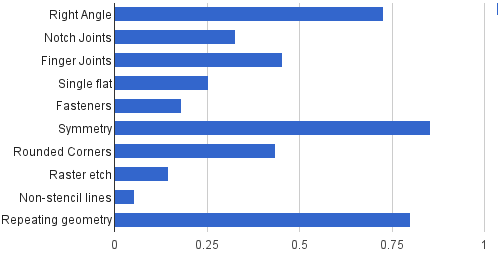
\includegraphics[width=0.9\linewidth]{img/ponoko-analysis.png}
  \caption{Frequency of certain attributes were present in laser-cut
    projects from Ponoko and Thingiverse.}
  \label{fig:ponoko}
\end{figure}

We used nine properties to characterize each project. These were
chosen based on our own experience with items made with laser cutters,
as well as from observations from the formative study (discussed
next). These properties are summarized here and described in greater
detail below:

\begin{itemize}
\item \textit{Right Angle}: Dominant edges meet at 90-degree angles.
\item \textit{Notch and Finger Joints}: Two parts come together using one of
  the joints illustrated in Figure~\ref{fig:joint}.
\item \textit{Single part}: Project is composed of a single, flat piece of
  material (e.g. a coaster).
\item \textit{Fasteners}: Clear use of glue, screws, or bolts.
\item \textit{Symmetry}: Radial or linear symmetry is a dominant feature.
\item \textit{Rounded Corners}: Right-angle corners are slightly blunt.
\item \textit{Raster etch}: Laser cutter etched patterns (e.g. words,
  images) rather than cutting all the way through material.
\item \textit{Repeating geometry}: Linework is repeated several times,
  often in a way that suggests procedural generation.
\end{itemize}

\begin{figure}[h]
\centering 
\subfloat[Notch joints.] {
  \label{fig:joint-notch} 
  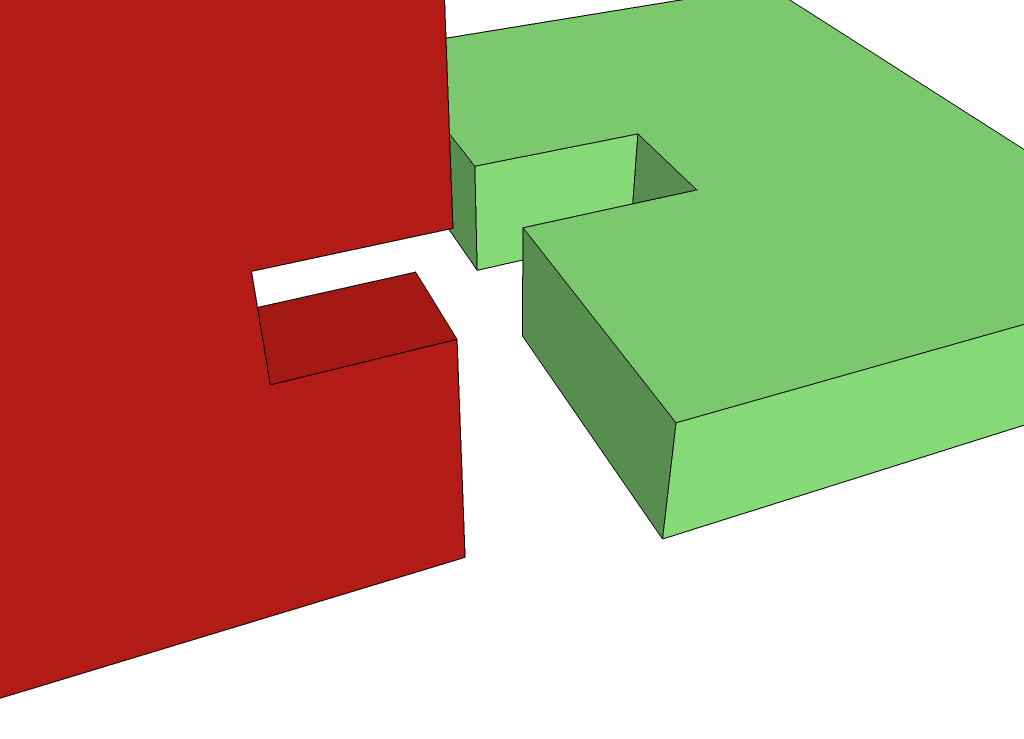
\includegraphics[width=0.4\linewidth]{img/joint-notch.png}
}
\subfloat[Finger joints, alternately called box joints.] {
    \label{fig:joint-finger}
    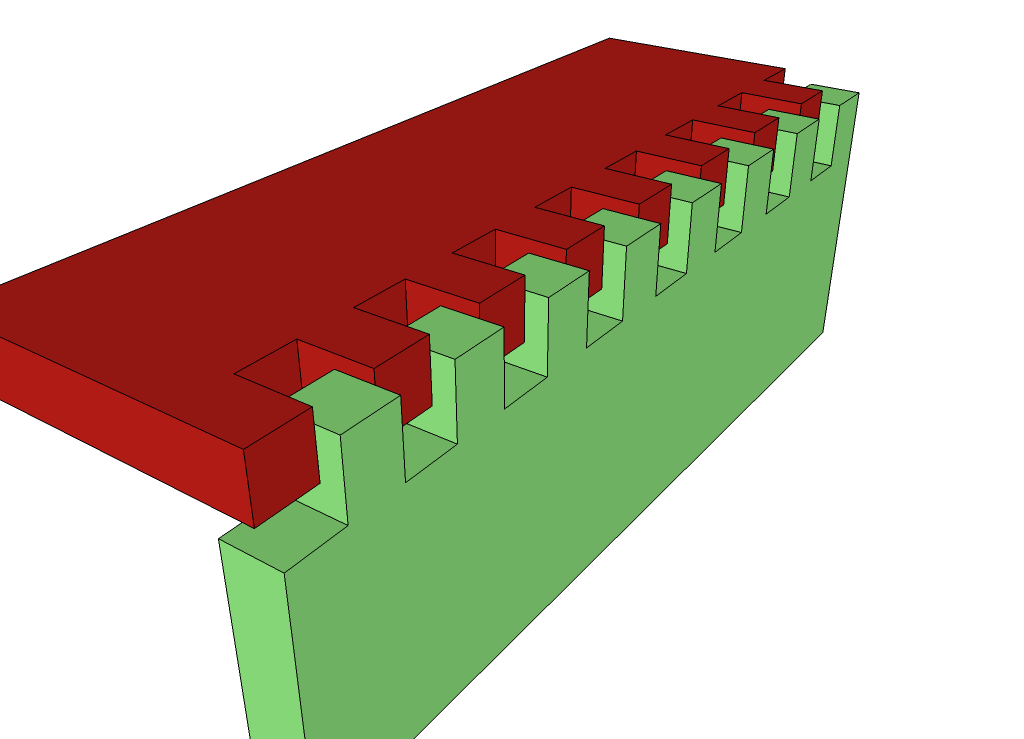
\includegraphics[width=0.4\linewidth]{img/joint-finger.png}
}
\caption{Two common joint types.}
\label{fig:joint}
\end{figure}

Single part projects were typically artistic, using expressive, curvy
linework. Among those objects composed of more than one piece,
approximately 75\% used finger or notch joints
(Fig.~\ref{fig:joint}). The rest used fasteners.

The more professional-looking models were generally those that used
rounded corners. Raster etching was also used in several cases for
artistic effect. Repeating geometry was found in most models. These
patterns involve sequences of lines or curves with consistent length
and angles. Some patterns were quite ornate.

\section{SKETCH IT, MAKE IT}

Based on observing of designer's work practices and the artifacts they
make, we have developed \textit{Sketch It, Make It} (SIMI), a
sketch-based tool for modeling laser cut items. We aim to address
problems with current modeling systems enumerated above in a tool that
specifically supports designing laser-cut items.

% * map problems from earlier (x y z) to solutions in simi

% * overview of interaction

SIMI users draw with a stylus and can use an offhand button for a few
actions. The system recognizes input as either geometric linework or
gestural commands. Linework includes straight lines, elliptical arcs,
splines, circles, and ellipses. 

Users issue commands to operate on linework by drawing gestures. Some
gestures are recognized and invoke immediately, such as the erase
(scribble) gesture. Others, such as a command to constrain segments be
the same length, are recognized after the user presses the button, or
after a timeout.

When the user draws a closed 2D path, the system recognizes it as a
stencil. Stencils are shapes that can be placed on the virtual laser
cutter bed. Several copies of a stencil can be added. The system
generates a vector file that can be sent directly to a laser cutter.

After cutting the stencils, the user can assemble them to their final
configuration. Figure~\ref{fig:laser-example} shows several examples
of projects made with SIMI.

\subsection{Implementation}

\begin{figure}[h]
\centering \subfloat[Automatic: merge when endcaps intersect
  (drawn in blue).] {
  \label{fig:latch-auto} 
  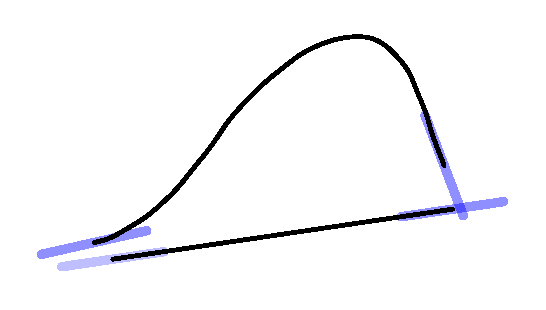
\includegraphics[width=0.43\linewidth]{img/latch-auto-endcaps.pdf}
}\hspace{5mm}
\subfloat[Latching endpoints.] {
  \label{fig:latch-endpoint} 
  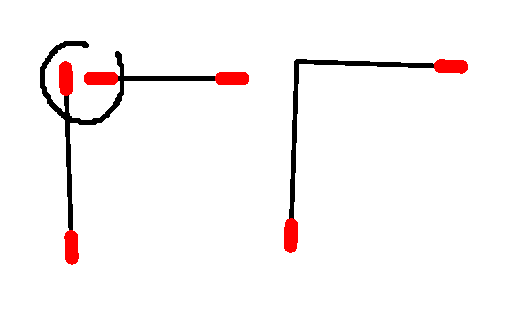
\includegraphics[width=0.43\linewidth]{img/latch-manual-endpoint.pdf}
}
\\
\subfloat[Latching continuation.] {
    \label{fig:latch-continuation}
    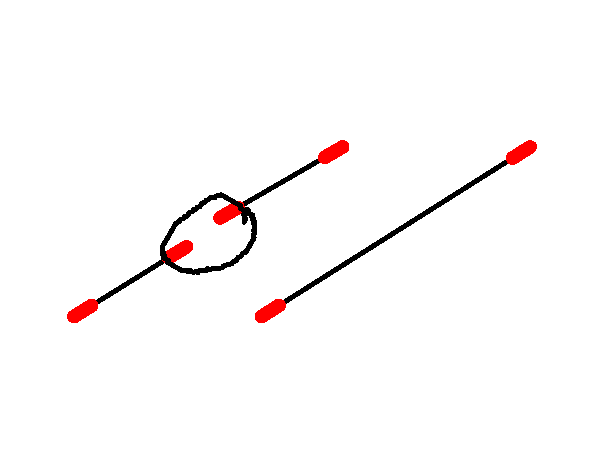
\includegraphics[width=0.43\linewidth]{img/latch-manual-continuation.pdf}
}\hspace{5mm}
\subfloat[Latching T-Junction.] {
    \label{fig:latch-tjunct}
    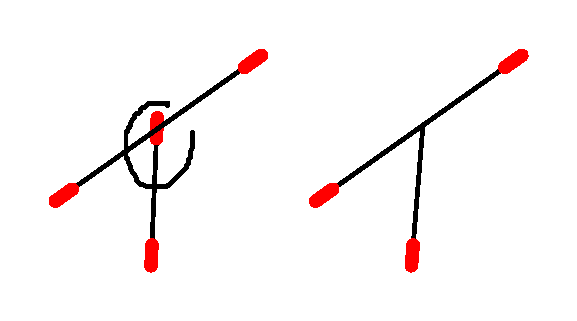
\includegraphics[width=0.43\linewidth]{img/latch-manual-tjunct.pdf}
}
\caption{Automatic and manual latching used to bring segments together.}
\label{fig:latch}
\end{figure}


%* Stylus with offhand button

The guiding principle we used when developing SIMI is that the
designer should never need to set down the pen. Input is provided
entirely with a stylus except for a single button used by the
non-dominant hand that gives access to additional commands. The
gestures used to invoke commands or add constraints are summarized
below.

\subsubsection{Latching}

Users often want adjacent lines to meet at a common point. Latching is
the process of combining adjacent segments (lines, splines, arcs,
\textit{etc.}) so they meet at a common point. For example, users may
draw a square with with four strokes, and eight unique pen-down/pen-up
locations, but a square should have only four corners.

SIMI provides two methods for latching segments, illustrated in
Figure~\ref{fig:latch}. One is automatic: the system analyzes new
linework for cases where the user probably meant their segments to
join together, and adjusts one or more segments to join. Automatic
latching can be problematic if it is too zealous. Early approaches
used only distance to find which segments should be
latched~\cite{herot-latch-corners}: if two endpoints were within $x$
units of one another, latch them. This works well when segment lengths
are large relative to $x$. But when the segments are short, the
latcher merges points that the designer intended to remain distinct.

SIMI's automatic latcher uses length and the segment direction at the
endpoint. It creates an \textit{endcap}: a line segment centered at an
end point that is a fraction of the line length (currently 0.1) that
follows the tangent at the end point. For nearby segments to latch
automatically, the related endcaps must intersect. SIMI can latch two
or more segments in this manner.

The automatic latching process is intentionally conservative to avoid
frustrating users. Therefore it is common for the automatic process to
miss some places where the user wanted lines to meet. Therefore SIMI
gives users a simple method to latch segments: draw a small circle
around the target endpoints.

All linework in SIMI is meant to compose stencils, which are sequences
of latched segments. Therefore the designer must be able to find
un-latched segments. The system draws a red marker at lonely endpoints
to expose un-latched segments.

Segments can be manually latched together in three ways: endpoint
latching, continuation, and T-junctions. Endpoint latching is what the
automatic latcher does. Continuation latching is when the user brings
together two segments that are close to the same direction at the
joined point. Continuation latching replaces two segments with a
single larger segment. A T-junction is when a segment endpoint latches
to the middle of another segment, splits the second segment in two.

\subsubsection{Erase}

\begin{figure}[h]
  \centering
  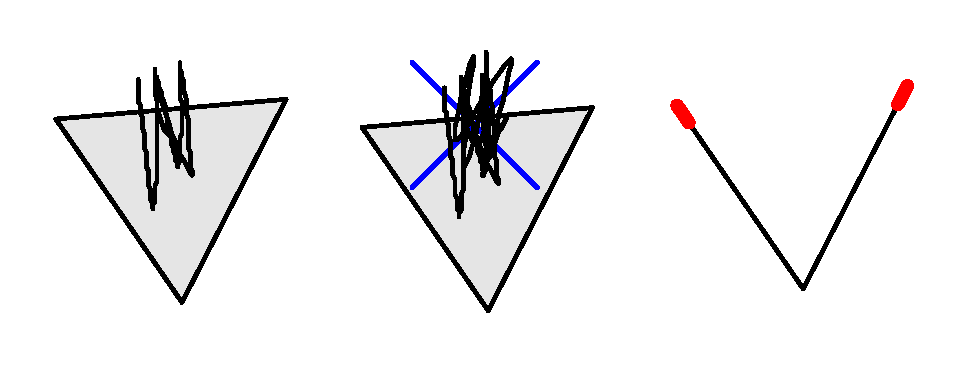
\includegraphics[width=0.9\linewidth]{img/erase-all.pdf}
  \caption{Erase gesture: before, during, and after.}
  \label{fig:erase}
\end{figure}

Users may want to remove linework for various reasons: deleting
unwanted or accidental items, or as part of a deliberate strategy to
cut away geometry to allow new shapes to
emerge~\cite{zeleznik-lineogrammer}. Like latching, erasing is a
common task so it is invoked with a simple scribble gesture. During
development we tried various algorithms for detecting erasure. The
first attempts were computationally intensive enough that they could
only be performed once after the pen was released. However, test users
found it difficult to perform the gesture correctly. Done wrong, the
input would be recognized as linework and remain on the canvas, which
users would need to erase using the same problematic algorithm. This
caused considerable frustration.

Our new algorithm for detecting erasure is easy to perform, and is
efficiently runs during as the pen stroke. When an erasure gesture is
detected mid-stroke, it provides visual feedback that gives users
confidence and avoids frustration. Figure~\ref{fig:erase} shows an
erase gesture with the visual feedback.

Erase (scribble) gestures are detected as follows. First we assign
each point $P_i$ with a time stamp $T_i$, a curvilinear distance
$D_i$, and a heading vector $H_i$. Curvilinear distance is the path
length along the stroke from the first point: $D_0$ is zero, and the
rest are $D_i = distance(P_{i-1}, P_i)$.

A pen stroke will not be considered an erasure if the pen has not
moved more than a minimum distance from the start point (we use 10
pixels).

The heading $H_i$ for point is a normalized vector from $P_{i-k}$ to
$P_{i+k}$, for a window size of some $k$ (we use $k=1$ but for higher
resolution input surfaces $k$ should be larger). The first $k$ points
use $H_k$ for their heading.

Next we add points to a list of samples $S$. If $D_i$ is more than
some threshold beyond the most recently added sample point, $P_i$ is
added to $S$. When a new sample point is added, it assembles a
sub-list $R$ of recent sample points that occurred within $t$
milliseconds (our implementation uses 100ms). If the angle between any
point in $R$ and the new point is greater than some value (we use
$\pi$ radians), it increments a `corner' count value for the current
pen stroke. When more than some number of corners is found for a
stroke, the system draws feedback to alert the user and halts
recognition until the pen is lifted.

Because the sample list depends on a relatively short time period, the
user must scribble with vigor to activate the erase gesture. If the
user intends to erase but draws slowly, they quickly learn that they
can just scribble a little faster and wait for the visual feedback.

\subsubsection{Undo and Redo}

Another way to recover from unwanted actions---particularly a sequence
of them---is to undo. Users undo by holding down the offhand button
and dragging the pen to the left. Every 40 pixels left triggers one
undo action. This lets the designer undo several actions by simply
dragging farther to the left. Redo is done by dragging to the
right. Both undo and redo actions can be triggered by the same stroke
by changing direction. This lets the designer seek a prior state by
dragging left and right.

\subsubsection{Right Angle and Length Constraints}

\begin{figure}[h]
  \centering
  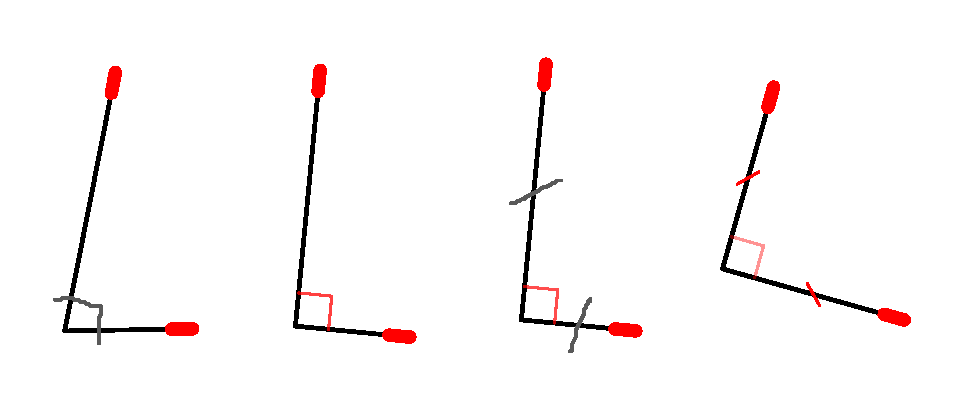
\includegraphics[width=0.9\linewidth]{img/constraints-all.pdf}
  \caption{Gestures for adding a right angle (left) and same-length.}
  \label{fig:constraints}
\end{figure}

Designers add geometric constraints via drawn gestures. In traditional
drafting and standard geometry diagrams, a brace symbol at the
intersection of the two edges indicates a right angle. SIMI recognizes
drawn input that looks like that brace and adds a constraint on the
associated segments. These are shown in
Figure~\ref{fig:constraints}. Erasing either segment in a right-angle
constraint also removes the constraint.

Another convention from drafting is to use tick marks to indicate that
two lengths are the same length. SIMI recognizes two or more ticks
crossing line segments as a gesture to create a \textit{same length
  constraint}. If the user hashes a line segment that is already
involved in a same-length constraint, that segment is added to the
existing constraint. Removing a segment involved in a same-length
constraint only deletes the constraint if it is the last one.

A same-length constraint is satisfied when all segment lengths are
even. The final length is the mean value of the initial lengths.

SIMI also lets designers set specific lengths. Currently this is
invoked by selecting a line (by over-tracing a portion of it) and
typing a number. Handwriting recognition would be preferred. If one of
the segments in a same-length constraint is assigned a particular
length, all segments take on that particular length.

\subsubsection{Flow Selection}

\begin{figure}[h]
\centering \subfloat[Selecting (``heating'') points along a curve near
  the stylus. The selection grows with time. ] {
  \label{fig:fs-1} 
  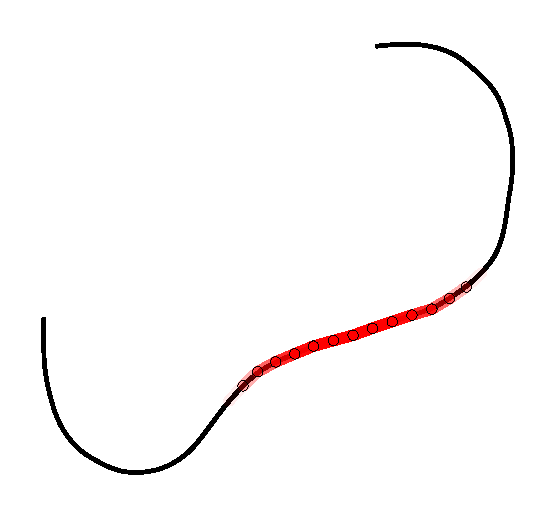
\includegraphics[width=0.4\linewidth]{img/fs-1.pdf} }
\hspace{3mm}
\subfloat[Deforming the heated region by moving the stylus.] {
  \label{fig:fs-2} 
  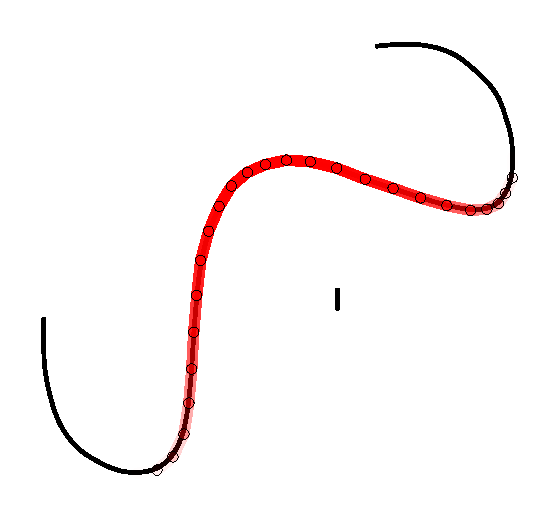
\includegraphics[width=0.4\linewidth]{img/fs-2.pdf}
}
\caption{Flow selection.}
\label{fig:fs}
\end{figure}

Flow selection~\cite{johnson-flow-selection} is a technique to
manipulate curves organically (Figure~\ref{fig:fs}). The user `heats
up' portions of curved segments by holding the pen down near the
curve. Then, without picking the pen up, the user moves the heated
region by dragging the pen. Points along the curve move more if they
are `hotter'.

% TODO: add to flow selection section.

\subsubsection{Reference Points and Guides}

\begin{figure}[h]
  \centering
  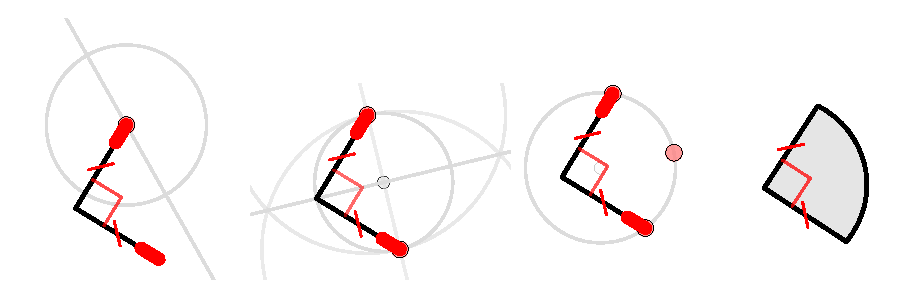
\includegraphics[width=0.9\linewidth]{img/guides-all.pdf}
  \caption{Reference points and guides. The first three panels show
    one, two, and three reference points and the guides that are
    displayed as a result. The designer uses the circular guide to
    create the circular arc shown in the final panel.}
  \label{fig:guides}
\end{figure}

The user may create handles to move segment endpoints around by
drawing `reference points'. These are dots made by swirling the pen
around in a tiny area (within 9 pixels) quickly (less than 500ms). The
user can then reposition reference points to adjust attached geometry.

When reference points are present, the system shows guides to aid
additional drawing. The possible combinations are illustrated in
Figure~\ref{fig:guides}. When there is one reference point, the system
uses the pen's hover location, drawing a circle centered at the
reference point, and a line passing through both. This can be used to
make a hole centered at a particular location.

Two reference points give the user three circles, two lines, and shows
the midpoint. Three reference points give the user a circle that
passes through them, and indicates that circle's center.

\subsection{Constraint Engine}

SIMI lets designers establish \textit{constraints} that enforce some
geometric relationship among items~\cite{borning-thinglab}. For
example, the user might draw a triangle and establish a right angle
constraint. No matter how the user manipulates the drawing (moving
vertices or changing segment lengths), the constraint engine ensures
that particular corner remains a right angle.

SIMI uses an iterative, numeric solver that minimizes the total error
of all constraints. A constraint's error is reported as how far each
related point must move to satisfy the constraint. However, points may
be involved in many constraints, so it is not generally possible to
simply move points to where they satisfy each constraint. To resolve
contending constraints, the system computes a change vector for each
point by polling each constraint. Each point is moved a small amount
along its change vector, and the process continues until the total
error becomes miniscule.

The solver can get trapped in a loop as points oscillate between
several values. We use simulated annealing to avoid this case: the
amount that points move varies randomly, and is larger when there is
more heat. Gradually the system `cools off' and the points settle in
to a satisfactory configuration.

Using a small number of primitive constraints on lengths and angles,
SIMI can create higher-level user constraints such as those that keep
segments at right angles or to be the same length.

\subsection{Stencils}

SIMI's final product is a ``cut file'': a vector drawing for a laser
cutter. This cut file typically contains a number of stencils, which
are closed 2D shapes that define the laser's path. Stencils may have
complex boundary geometry with non-intersecting edges. Stencils can
also have any number of holes in them, which could be used for joints,
fasteners, or some other purpose.

To identify stencils, SIMI forms a graph with segment endpoints as
nodes and segments as edges. It then runs a depth-first search. The
longest path that forms a cycle from a given point is considered a
possible stencil. After completing the search, only the longest paths
are kept. Stencils are visually represented by shading the
interior. 

\section{EVALUATION}

* screenshots/photos from user study

* other results from user study...

\section{ACKNOWLEDGMENTS}

For those about to rock, we salute you.

% TODO: fill this in later. Leave left blank for blind review.

\bibliography{simi}

\end{document}
